\section{Data}
\label{chap:data}
In this section, we describe the data which were used to proof that our approach for the automatic optimized creation of railway timetables performes. For practical reasons we used the year 2013 as a reference year.\\
In section 3.1 the data for creating a timetable in advance are described and section 3.2 the ad-hoc requests coming in via a digital app.

\subsection{Data Netzfahrplan}
\label{chap:dataFinVe}
To create a timetable in advance you need several input data for the Konstruktions and Belegungs part, which are described in this section. \\
For the Konstuktion part we need the infrastructure on which we want to create the timetable and all requirements for the slot, the so called "Systemtrassenanforderungen", which defines the network where the automatic timetable takes place, the standardized train characteristics and the daily load curve. 

\subsubsection{Infrastructure}
The infrastructure represents the digital representation of the german railyway network. It contains all information which are needed to construct an timetable, e.g. the priorities of the track or the length of an freight stop.\\
\textbf{\textcolor{red}{Mir ist nicht ganz klar, was hier alles aufgeschrieben werden muss... Oder reicht dies bereits?}}

\subsubsection{Systemtrassenanforderungen}
The requirements of systemization defines first of all the systemized network where automatic timetabling takes place (STA-Abschnitte), second it defines the charakteristics of the standardized trains (STA-Charakteristik) and last the daily load curve ("Tagesganglinie") which defines the pattern we want to schedule the trains.

\begin{itemize}
	\item[1)] STA-Abschnitt \\
	The STA-Abschnitte define the systemized network. A section of the germany railway network will be assigned to the systemized network if the section is part of the european rail freight corridor, if there are at least 48 freight trains per day on the section or if a logical completion of the network is nesessary. \\
	As a consequent, the systemized network maps 27\% of the german rail network based on the network length in kilometers. However, this covers 80\% of the freight transport demand. 
	%The start and end point of one STA Abschnitt should be in one railway station where one train has the opportunity to synchronize with another one. Hence, one Sytemtrasse can wait in that railway station for another.  
	
	\textbf{\textcolor{red}{Falls noch Platz, könnte hier die STA-Karte eingefügt werden}}
	\begin{figure}[h]
	\centering
	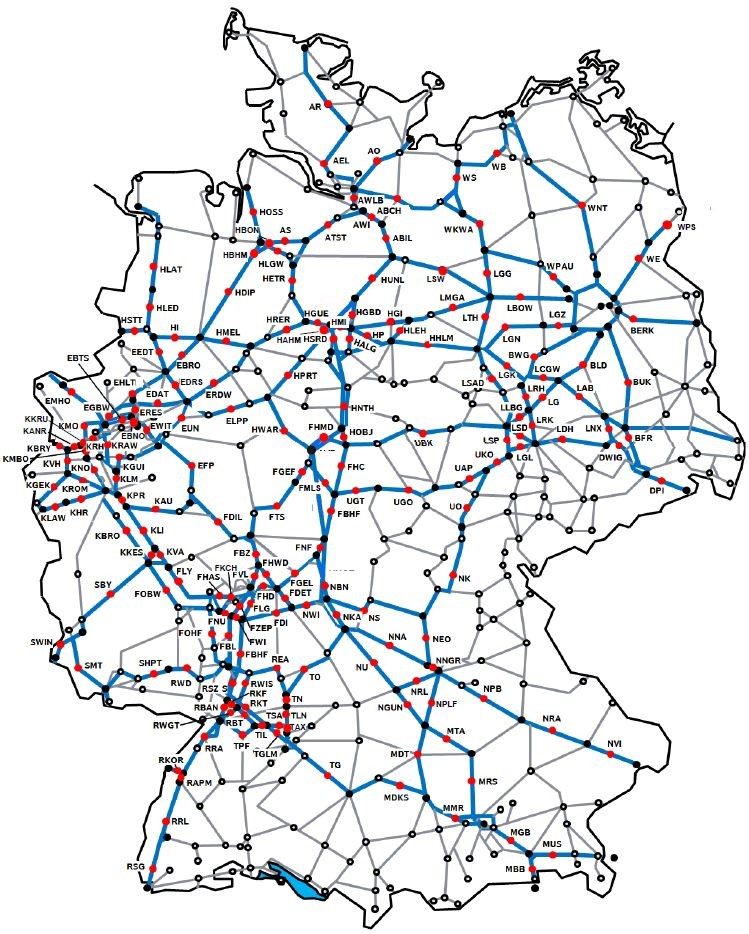
\includegraphics[width=0.7\textwidth]{Bilder/STA-Karte.jpg}
	\caption{The blue edges show the systemized network}
	\end{figure}
	
	\item[2)] STA-Characteristic \\
	The STA-Charakteristics define the standardized charakteristics on the systemized network. They were created by breaking down the forecast of the customers' request for the specific year. \\
	One systenmized network can have up to approximately 30 different charakteristiks. Where one STA-Abschnitt has up to three different ones. We limited the number of Charakteristics within the systemamized network as well as on one STA-Abschnitt since the synchronization within the Systemtrassen will be easier. 
	
	\item[3)] Tagesganglinie \\
	The daily load curve describes how many trains of one specific characteristic are suppose to be constructed in one time intervall. 
\end{itemize}

\subsubsection{Passenger Transport}
As our approach is for freight traffic only, the passenger transport is also an important input data. This data comes from the productive train scheduling programm of the german railway company. \\ 
\\
For the Belegungspart the actual customers' requests and the Systemtrassen are needed. A customers' request consists of the information from where to where he wants to drive, where the train has to stop, the charakteristic of the train and so on.\\

\textcolor{blue}{Customer Requests consist of the running points, time requirements and the characteristics of the train. The running points are at least the start of the request and its goal, but may also include some stops which should be served in between. The time requirements for our data consists only of an interval at the start of the request. But it is also possible to provide further time restrictions on the other running points. The characteristics of the request include all data necessary to calculate its dynamic properties such as acceleration and its static parameters like length, width and mass of the requested train.}

\textcolor{blue}{The difference between the two use cases is the set of customer requests. For the Netzfahrplan the set is fixed and equals all those trains which were requested for November, 14th 2013. In contrast, for the app only one request is provided to the algorithms at a time.}


\subsection{Data for Click \& Ride App}
\label{chap:dataCnR}
Since for the the Click \& Ride App we do not use Systemtrassen the only input data are the customers' requests. 
\\
\textbf{\textcolor{red}{Tue mir etwas schwer, was ich dort noch alles schreiben soll? Auch, weil ich nicht genau weiß, wo wir die Grenze zwischen dem Use Case und den Daten ziehen wollen.}}